\documentclass[10pt]{article}
\usepackage[english,russian]{babel}
\usepackage{textcomp}
\usepackage[left=2cm, right=2cm, top=1.5cm, bottom=1.5cm]{geometry}
\usepackage{tikz}
\usepackage{multicol}
\usepackage{hyperref}
\usepackage{amsmath}
\usepackage{listings}
\usepackage{colortbl}
\usepackage{graphicx}
\usepackage[shortlabels]{enumitem}
\usepackage{hyperref}
\pagenumbering{gobble}

\lstdefinestyle{CStyle}{
  language=C,
  basicstyle=\linespread{1.1}\ttfamily,
  basewidth=0.5em,
  texcl=true,
  keywordstyle=\color{blue}\bfseries,
  commentstyle=\color{gray},
  stringstyle=\ttfamily\color{orange!50!black},
  showstringspaces=false,
  backgroundcolor=\color{white},
  breaklines=true,
  breakatwhitespace=true,
  xleftmargin=5mm,
  keepspaces = true,
  extendedchars=\true,
  tabsize=4,
  upquote=true,
  emph={size_t, NULL},
  emphstyle={\color{blue}\bfseries},
}
\lstdefinestyle{boxStyle}{
  style=CStyle,
  framexleftmargin=5mm, 
  frame=shadowbox, 
  rulesepcolor=\color{gray}
}
\lstset{style=CStyle}

\renewcommand{\thesubsection}{\arabic{subsection}}
\makeatletter
\def\@seccntformat#1{\@ifundefined{#1@cntformat}%
   {\csname the#1\endcsname\quad}
   {\csname #1@cntformat\endcsname}}
\newcommand\section@cntformat{}
\newcommand\subsection@cntformat{Задача \thesubsection.\space}
\newcommand\subsubsection@cntformat{\thesubsubsection.\space}
\makeatother


\begin{document}
\title{Семинар \#4: Часть 2: Структуры. Домашнее задание.\vspace{-5ex}}\date{}\maketitle

\subsection{Треугольник}
Для описания точек и треугольников на плоскости были определены структуры \texttt{Point} и \texttt{Triangle}:
\begin{lstlisting}
#include <stdio.h>

struct point 
{
    double x
    double y;
};
typedef struct point Point;

struct triangle 
{
    Point a;
    Point b;
    Point c;
};
typedef struct triangle Triangle;

// Тут нужно написать все необходимые функции

int main()
{
    Triangle t = {{1.00, 0.00}, {0.50, 2.00}, {0.00, 1.50}};
    printf("Perimeter = %.2f\n", get_triangle_perimeter(&t));
    
    Point d = {1.0, 1.0};
    print_triangle(&t);
    move_triangle(&t, d);
    print_triangle(&t);
}

\end{lstlisting}
Напишите следующие функции для работы с этими структурами:
\begin{itemize}
\item Функцию \texttt{print\_point}, которая будет принимать точку и печатать её в формате \texttt{(1.23, 4.56)}. То есть в круглых скобках, через запятую и с двумя знаками после запятой.

\item Функцию \texttt{print\_triangle}, которая будет принимать на вход треугольник и печатать координаты треугольника в следующем формате: \texttt{\{(1.00, 0.00), (0.50, 2.00), (0.00, 1.50)\}}.

\item Функцию \texttt{distance}, которая будет принимать на вход 2 точки и возвращать расстояние между ними.

\item Функцию \texttt{get\_triangle\_perimeter}, которая будет принимать треугольник по константному указателю и возвращать его периметр.

\item Функцию \texttt{moved\_triangle}, которая будет принимать на вход треугольник по константному указателю и одну точку (она будет играть роль вектора-перемещения). Функция должна возвращать новый треугольник, у которого все координаты будут передвинуты на вектор-перемещение.

\item Функцию \texttt{move\_triangle}, которая будет принимать на вход треугольник по указателю и одну точку (она будет играть роль вектора-перемещения). Функция должна менять передаваемый ей треугольник.
\end{itemize}

\newpage
\subsection{Одна строка}
Решения всех подзадач этой задачи -- одна строка. Вам нужно создать файл в формате \texttt{.txt} и, используя любой текстовый редактор, записать в него ответы на все подзадачи. После этого, файл нужно поместить в ваш репозиторий на github.

\begin{enumerate}

\item В следующей программе создаётся структура \texttt{Book}:
\begin{lstlisting}
struct book 
{
    char title[50];
    int pages;
    float price;
};
typedef struct book Book;

int main() 
{
    Book b = {"Fahrenheit 451", 400, 700.0};
    
}
\end{lstlisting}
\begin{enumerate}
\item Создайте указатель \texttt{pb} и сделайте так, чтобы он указывал на структуру \texttt{b}.
\item Создайте указатель \texttt{pprice} и сделайте так, чтобы он указывал на поле \texttt{price} структуры \texttt{b}.
\item Создайте указатель \texttt{pc} и сделайте так, чтобы он указывал символ \texttt{'t'} поля \texttt{title} структуры \texttt{b}.
\end{enumerate}



\item В следующей программе была создана структура \texttt{a} типа \texttt{Movie} и указатель на неё.
\begin{multicols}{2}
\begin{lstlisting}
#include <stdio.h>
struct date 
{
    int day; 
    int month;
    int year;
};
typedef struct date Date;

struct movie 
{
    char title[50];
    float rating;
    Date release_date;
};
typedef struct movie Movie;
\end{lstlisting}
\vfill \null  
\columnbreak
\vfill \null  
\begin{center}
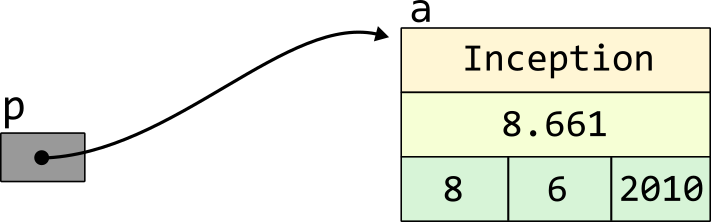
\includegraphics[scale=1]{../images/pointer_schemes/pointer_to_struct_movie.png}
\end{center}
\end{multicols}
\vspace{-10ex}
\begin{lstlisting}
int main() 
{
    Movie a = {"Inception", 8.7, {8, 6, 2010}};
    Movie* p = &a;
    
}
\end{lstlisting}
\begin{enumerate}
\item Увеличьте на \texttt{1} значение поля \texttt{rating}, используя только указатель \texttt{p}.
\item Увеличьте на \texttt{1} значение поля месяца выхода фильма, используя только указатель \texttt{p}.
\end{enumerate}



\item В следующей программе был создан массив \texttt{array} из структур типа \texttt{Movie} и указатель \texttt{p}, который указывает на второй элемент массива (\texttt{array[1]}).
\begin{lstlisting}
#include <stdio.h>
struct date 
{
    int day;
    int month;
    int year;
};
typedef struct date Date;

struct movie 
{
    char title[50];
    float rating;
    struct date release_date;
};
typedef struct movie Movie;

int main() 
{
    Movie array[3] = {{"Inception", 8.661, {8, 6, 2010}}, 
                      {"Green Mile", 9.062, {6, 12, 1999}}, 
                      {"Leon", 8.679, {14, 9, 1994}}};
    Movie* p = &array[1];
}
\end{lstlisting}

\vspace{-55ex}
\begin{center}
\quad\quad\quad\quad\quad\quad\quad\quad\quad\quad\quad\quad\quad\quad\quad\quad\quad\quad\quad\quad\quad\quad\quad
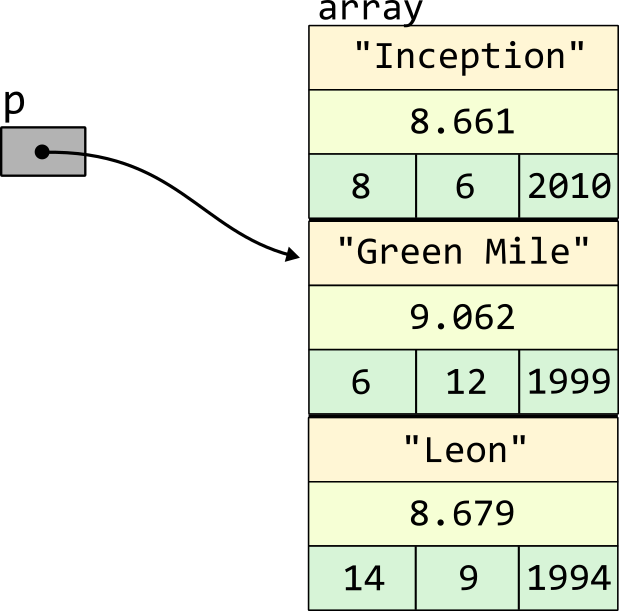
\includegraphics[scale=1]{../images/pointer_schemes/pointer_to_array_of_struct_movie.png}
\end{center}

\begin{enumerate}
\item Увеличьте на \texttt{1} значение рейтинга фильма \texttt{Inception}, используя только указатель \texttt{p}.
\item Удвойте значение года выхода фильма \texttt{Leon}, используя только указатель \texttt{p}.
\end{enumerate}
\end{enumerate}




\subsection{Рецензии на компьютерные игры}
На вход программе приходит информация о рецензиях компьютерных игр. В первой строке содержится число \texttt{n} - количество игр. Далее идут \texttt{n} строк. В каждой строке содержится название игры, заканчивающееся двоеточием сразу после идёт целое число \texttt{k} -- количество оценок, которые эта игра получила, затем идут \texttt{k} оценок. Оценка, это число от 1 до 10. Нужно отсортировать все игры по средней оценке и напечатать название игр и их среднюю оценку.

\begin{center}
\begin{tabular}{ l | l }
 вход & выход \\ \hline
 \texttt{5} & 								  \texttt{The Cube, 8.286} \\
 \texttt{Need For Speed: 6 6 1 2 7 5 4} &      \texttt{Metal Power, 5.900 } \\
 \texttt{Sector: 3 1 4 2} & 					  \texttt{Principle Of Chaos 2, 5.200} \\
 \texttt{The Cube: 7 9 8 7 9 8 10 7} &          \texttt{Need For Speed, 4.667 } \\
 \texttt{Principle Of Chaos 2: 5 4 3 6 5 7} &     \texttt{Sector, 2.333} \\
 \texttt{Metal Power: 10 8 5 3 9 6 2 6 7 5 8} & \\
\end{tabular}
\end{center}
Для считывания до символа \texttt{:} можно использовать \texttt{scanf} следующим образом:
\begin{lstlisting}
char title[50];
char temp;
scanf("%[^:]", title);  // Считываем название до символа :
scanf("%c", &temp);     // Считываем символ :
...                     // Считываем числа
scanf("%c", &temp);     // Считываем перенос на новую строку ( символ \textbackslash n )
scanf("%[^:]", title);  // Считываем название до символа :
scanf("%c", &temp);     // Считываем символ :
...
\end{lstlisting}
Протестировать программу можно на файле \texttt{videogames.txt}.



\subsection{Выравнивание типов}
Напишите программу, которая будет печатать на экран размеры и выравнивания следующих типов:

\begin{multicols}{2}
\begin{enumerate}
\item \texttt{char} 
\item \texttt{int} 
\item \texttt{size\_t} 
\item \texttt{int[10]} 
\item \texttt{int*} 
\item \begin{verbatim}
struct cat
{
    char x;
    size_t y;
};
\end{verbatim}

\item \begin{verbatim}
struct dog
{
    size_t y;
    char x;
};
\end{verbatim}

\item \begin{verbatim}
struct mouse
{
    char x;
    char y;
    size_t z;
};
\end{verbatim}

\item \begin{verbatim}
struct rat
{
    char x;
    size_t z;
    char y;
};
\end{verbatim}

\item \begin{verbatim}
struct fox
{
    char x;
    struct mouse y;
};
\end{verbatim}
\end{enumerate}
\end{multicols}

\subsection{Зацикленные структуры}
Пусть есть структура \texttt{Node}, которая хранит некоторое число и указатель на такую же структуру \texttt{Node}:
\begin{lstlisting}
struct node
{
    int value;
    struct node* ptr;
};
typedef struct node Node;
\end{lstlisting}
Напишите программу, которая будет создавать две такие структуры и инициализировать их поля значениями, показаными на рисунке:
\begin{center}
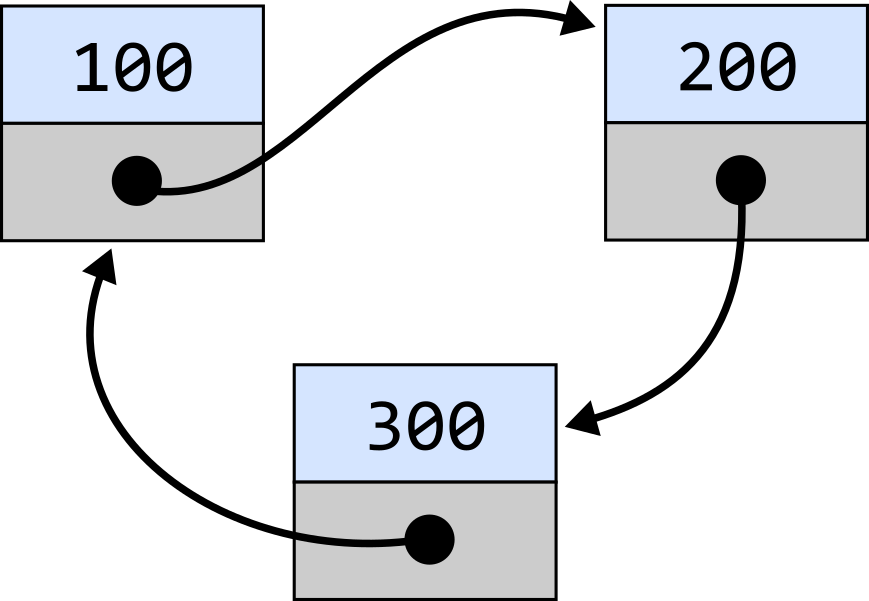
\includegraphics[scale=0.8]{../images/cycle2.png}
\end{center}
Указатель \texttt{ptr} первой структуры должен указывать на вторую структуру, а указатель \texttt{ptr} второй структуры, должен указывать на третью структуру, а указатель третьей -- на первую.

Напишите программу, которая будет печатать значение \texttt{value} структуры, а потом переходить к следующей структуре через поле \texttt{ptr}, потом печатать значение \texttt{value} уже этой структуры и переходить по полю \texttt{ptr} к следующей и так далее до бесконечности.

\newpage
\section*{Необязательные задачи (не входят в ДЗ, никак не учитываются)}
\setcounter{subsection}{0}


\subsection{Передача в функцию по указателю}
\subsection*{Передача в функцию по значению}
\begin{multicols}{2}
\begin{lstlisting}
#include <stdio.h>
struct movie 
{
    char title[50];
    float rating;
    struct date release_date;
};
typedef struct movie Movie;

void change_rating(Movie m) 
{
    m.rating += 1;
}
int main() 
{
    Movie a = {"Inception", 8.661, 
                {8, 6, 2010}};
    change_rating(a);
}
\end{lstlisting}
\columnbreak
\begin{center}
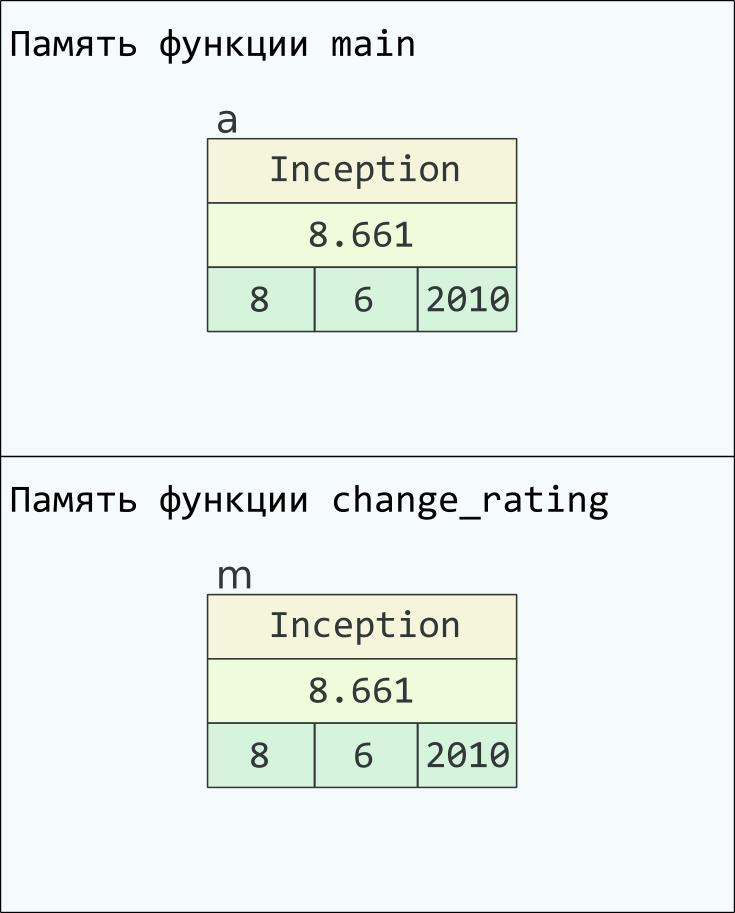
\includegraphics[scale=0.8]{../images/pointer_schemes/function_by_value.png}
\end{center}
\end{multicols}
Всё, что передаётся в функцию, копируется (кроме массивов). Поэтому функция \texttt{change\_rating} будет менять
поле \texttt{rating} у копии структуры \texttt{a}, а изначальная структура не изменится.

\subsection*{Передача в функцию по указателю:}
\begin{multicols}{2}
\begin{lstlisting}
#include <stdio.h>
struct movie 
{
    char title[50];
    float rating;
    struct date release_date;
};
typedef struct movie Movie;

void change_rating(Movie* pm) 
{
    pm->rating += 1;
}
int main() 
{
    Movie a = {"Inception", 8.661, 
              {8, 6, 2010}};
    Movie* p = &a;
    change_rating(&a);
}
\end{lstlisting}
\columnbreak
\begin{center}
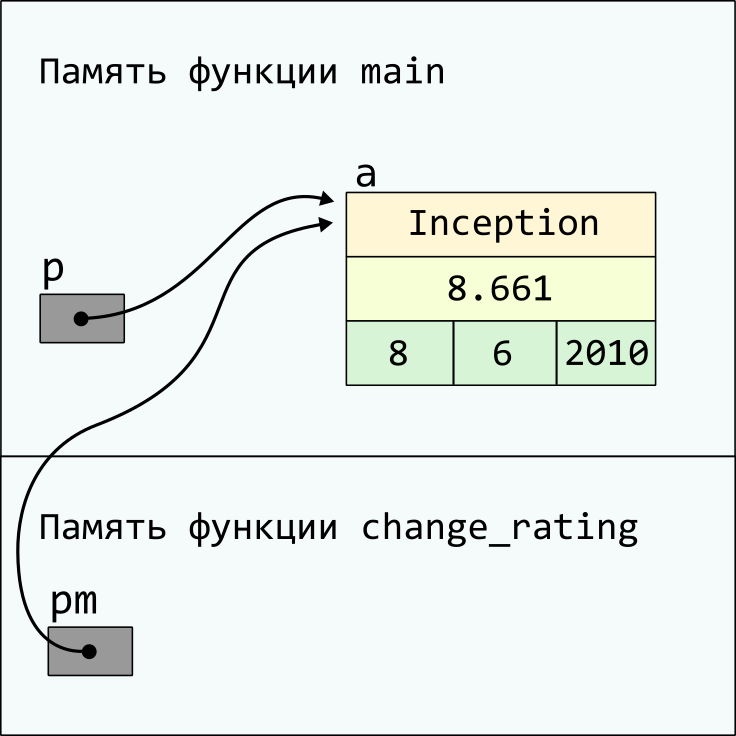
\includegraphics[scale=0.8]{../images/pointer_schemes/function_by_pointer.png}
\end{center}
\end{multicols}
Теперь в функцию копируется указатель, который содержит
адрес стурктуры \texttt{a}. Используя этот указатель, мы можем изменить изначальную структуру. Более того, так как указатель занимает меньше памяти, его копирования в функцию происходит быстрее, чем копирование всей структуры.

\subsection*{Подзадачи:}
\begin{enumerate}

\item Напишите функцию \texttt{void increase\_rating(Movie* p)}, которая будет принимать указатель типа \texttt{Movie*} и увеличивать рейтинг фильма, на которой указывает \texttt{p}, на 1.

\item Напишите функцию \texttt{void change\_year\_of\_movies(Movie* p, int size)}, которая принимает на вход указатель на первый элемент массива структур типа \texttt{Movie} и размер этого массива. Функция должна увеличивать год выхода всех фильмов на \texttt{1}. Протестируйте функции, вызвав их из функции \texttt{main} с помощью следующего кода:

\begin{lstlisting}
#include <stdio.h>
struct date 
{
    int day, month, year;
};
typedef struct date Date;
struct movie 
{
    char title[50];
    float rating;
    struct date release_date;
};
typedef struct movie Movie;

void print_date(const Date* pd) 
{
    printf("%02d.%02d.%04d", pd->day, pd->month, pd->year);
}
void print_movie(const Movie* pm) 
{
    printf("Title: %s\nRating: %.2f\nDate: ", pm->title, pm->rating);
    print_date(&pm->release_date);
    printf("\n");
}
// Тут вам нужно написать функции increase\_rating и change\_year\_of\_movies

int main() 
{
    Movie a[3] = {{"Inception", 8.661, {8, 6, 2010}}, 
                  {"Green Mile", 9.062, {6, 12, 1999}}, 
                  {"Leon", 8.679, {14, 9, 1994}}};
    increase_rating()
    change_year_of_movies(a, 3);
    for (int i = 0; i < 3; ++i)
        print_movie(&a[i]);
}
\end{lstlisting}

\end{enumerate}
\end{document}